% question 3
\section{Question 3}
\paragraph{(a)} Dynamic model is given by
\begin{align*}
I_1 \ddot{\theta}_1 &= \tau - K(\theta_1 - \theta_2) - D(\dot{\theta}_1 - \dot{\theta}_2), 
\\
I_2 \ddot{\theta}_2 &= K(\theta_1 - \theta_2) + D(\dot{\theta}_1 - \dot{\theta}_2), 
\end{align*}
\noindent where $K$ is stiffness and $D$ is damping.


\paragraph{(b)} Transfer functions are:
\begin{align*}
G_1(s) &=\frac{\theta_1(s)}{\tau(s)} = \frac{I_2 s^2 + Ds + k}{I_1 I_2 s^4 + s^3(I_1 D + I_2 D) + s^2 (I_1 K + I_2 K) }, \\ 
G_2(s) &=\frac{\theta_2(s)}{\tau(s)} = \frac{Ds + k}{I_1 I_2 s^4 + s^3(I_1 D + I_2 D) + s^2 (I_1 K + I_2 K) }.
\end{align*}


\paragraph{(c)} Figure \ref{fig:q3_OL} describes time-response of open-loop systems ($G_1(s)$ and $G_2(s)$) for different values of stiffness ($K=10^{-1}[1, 1.4, 1.8, 2.2, 2.6, 3]$ $\mathrm{\frac{N.m}{rad}}$) and damping ($D=10^{-3}[1, 1.8, 2.6, 3.4, 4.2, 5]$ $\mathrm{\frac{N.m.s}{rad}}$).

\begin{figure}[h!]
\centering
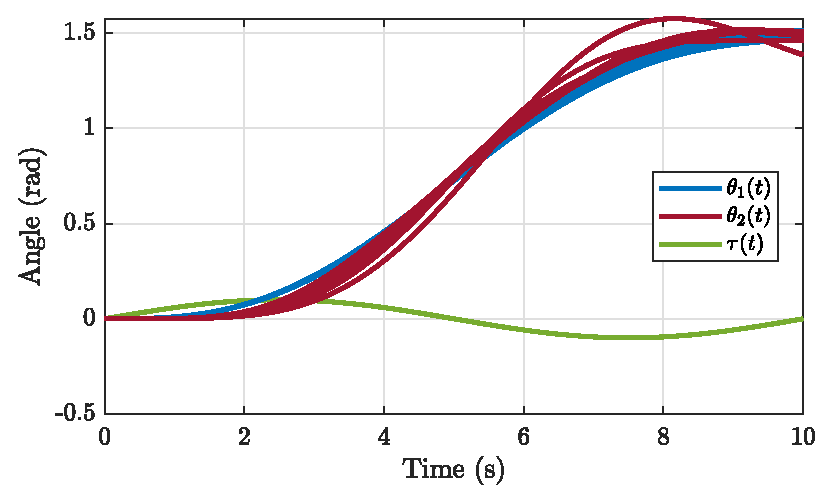
\includegraphics{images/question3/q3_OL.eps}
\caption{Time-response of open-loop systems ($G_1(s)$ and $G_2(s)$) considering sinusoidal input ($\tau=0.1\sin{0.2\pi t}$) and different values of stiffness and damping ($K=10[1, 1.4, 1.8, 2.2, 2.6, 3]$ $\mathrm{\frac{N.m}{rad}}$ and $D=1000[1, 1.8, 2.6, 3.4, 4.2, 5]$ $\mathrm{\frac{N.m.s}{rad}}$). }
\label{fig:q3_OL}
\end{figure}


\paragraph{(d)} On one hand, Figure \ref{fig:q3_rlocus_K_CL} describes root-locus of close-loop system with proportional gain. In this figure, third and fourth poles ($p_3, p_4$) are located in the right half-plane for any proportional gain value. On the other hand, Figure \ref{fig:q3_bode_K_OL} describes bode diagram of open-loop system ($G_2(s)$). In this figure, gain margin is $G_m=-13$ dB and phase margin is $P_m=179^{\circ}$. Likewise, phase diagram is below $-180^{\circ}$, thus gain margin will be negative for any proportional gain value. In conclusion, both root-locus and frequency response method indicates that close-loop system cannot be controlled with just a proportional gain.

\begin{figure}[h!]
\centering
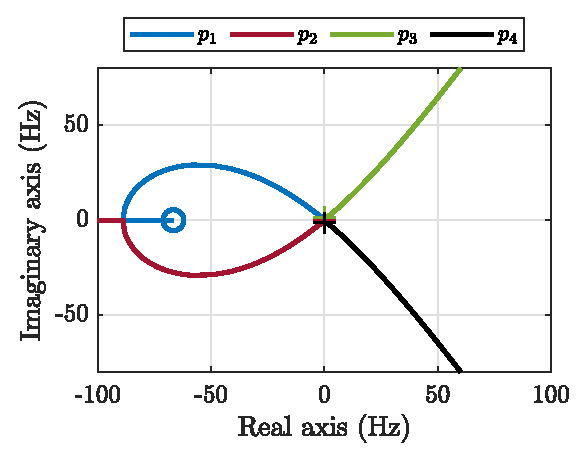
\includegraphics{images/question3/q3_rlocus_K_CL.eps}
\caption{Root-Locus of close-loop system with proportional gain.}
\label{fig:q3_rlocus_K_CL}
\end{figure}


\begin{figure}[h!]
\centering
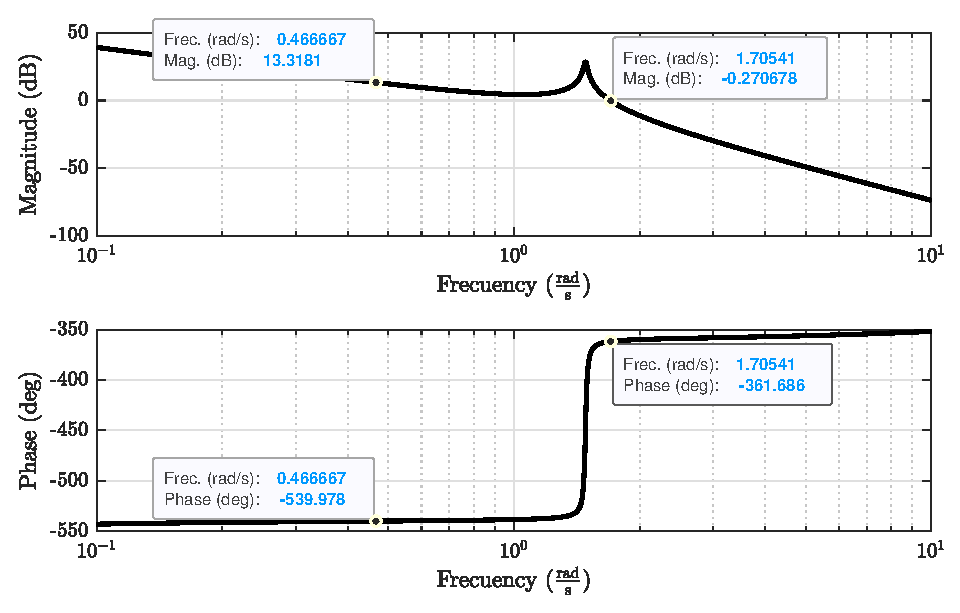
\includegraphics{images/question3/q3_bode_K_OL.eps}
\caption{Frequency response of open-loop system $G_2(s)=\frac{\theta_2(s)}{\tau(s)}$.}
\label{fig:q3_bode_K_OL}
\end{figure}



\paragraph{(e)} On one hand,  Figure  \ref{fig:q3_rlocus_KD_CL} describes root-locus of close-loop system with proportional-derivative gain. In this figure, poles are located in the left half-plane for proportional gain from $0.0001$ to $0.275$ and derivative gain from $0.00001$ to $0.0275$; then, first and second poles ($p_1, p_2$) move to right half-plane and close-loop system becomes unstable. On the other hand, Figure \ref{fig:q3_bode_KD_OL} describes bode diagram of open-loop system with proportional-derivative control method. In this figure, gain margin is greater than $0$ dB for proportional and derivative gains lower than $0.275$ and $0.0275$, respectively. Likewise, gain margin is lower than $0$ dB (close-loop system unstable) when resonance peak is above $0$  dB. 


\begin{figure}[h!]
	\centering
	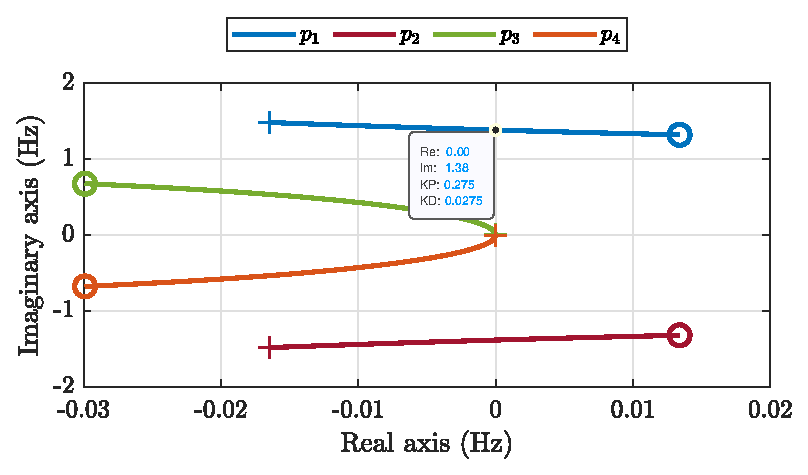
\includegraphics{images/question3/q3_rlocus_KD_CL.eps}
	\caption{Closed-loop system pole location diagram with proportional-derivative control method. Likewise, information box indicates maximum proportional and derivative gains until system becomes unstable.}
	\label{fig:q3_rlocus_KD_CL}
\end{figure}


\begin{figure}[h!]
	\centering
	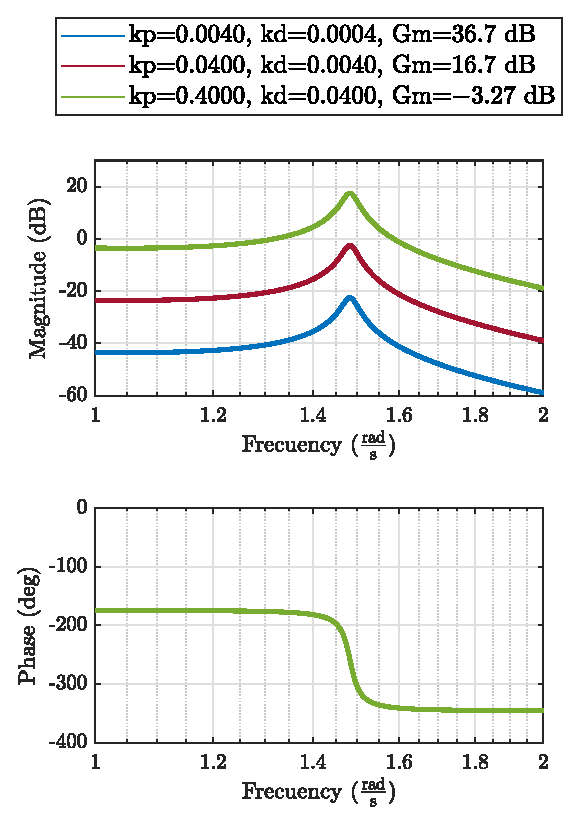
\includegraphics{images/question3/q3_bode_KD_OL.eps}
	\caption{Frequency response of open-loop system $G_{PD}(s) G_2(s)$.}
	\label{fig:q3_bode_KD_OL}
\end{figure}

\newpage
\paragraph{(f)}  Figure \ref{fig:q3_rlocus_KD_CL} indicates that close-loop system have imaginary poles two times. On one hand, at the beginning (control gains: $k_p=0.0001$ and $k_d=0.0001$), third and fourth poles are $+0.0095i$ and $-0.0095i$, respectively. On the other hand, at the middle  (control gains: $k_p=0.275$ and $k_d=0.0275$), first and second poles are $+1.3832i$ and $-1.3832i$, respectively. Likewise,  close-loop system is stable for proportional gain from $0.0001$ to $0.275$ and derivative gain from $0.00001$ to $0.0275$, thus, the proportional gain $kp=0.04$ and derivative gain $kd=0.004$ will be used. 

Then, poles are:
\begin{align*}
	p_1=&-0.0146 + 1.4706i, \\
	p_2=&-0.0146 - 1.4706i, \\
	p_3=&-0.0019 + 0.1923i, \\
	p_4=&-0.0019 - 0.1923i ,
\end{align*}
\noindent dominant poles are $p_3$ and $p_4$ because they are more closer to $0$. Hence, Figure \ref{fig:q3_step_KD_CL} describes step response of close-loop system and time characteristic are:
\begin{align*}
	\%PO &= 100 \%, \\
	Ts &= 2480 \textrm{ } \mathrm{s}. 
\end{align*}

\begin{figure}[h!]
	\centering
	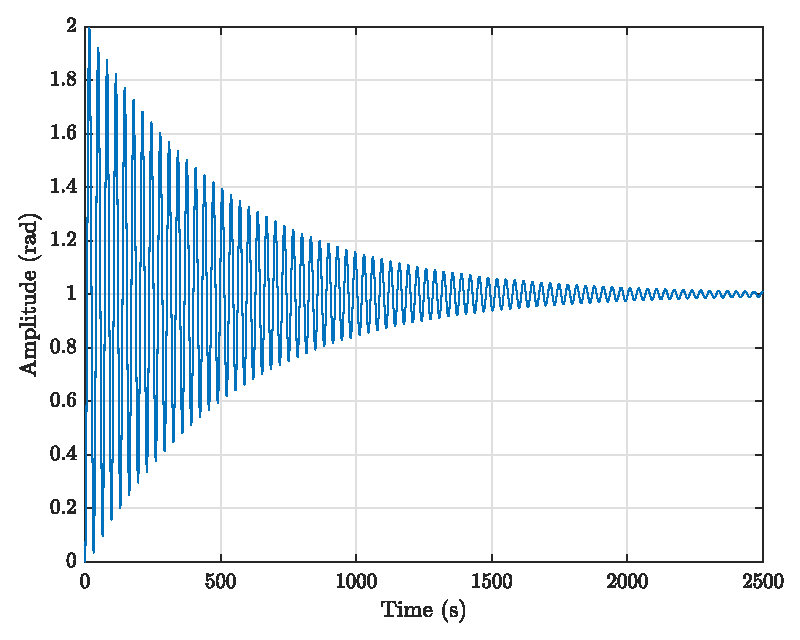
\includegraphics{images/question3/q3_step_KD_CL.eps}
	\caption{Step response of close-loop system with proportional-derivative control method (control gains: $k_p = 0.04$ and $k_d=0.004$).}
	\label{fig:q3_step_KD_CL}
\end{figure}

\newpage
\paragraph{(g)} Figure \ref{fig:notch_filter} describes bode diagram of Notch filter $N(s)=\frac{s^2 + 1}{(s+10)^2}$. On one hand, magnitude graph indicates that filter will help to increase gain margin of close-loop system. On the other hand, phase graph indicates that filter will help to increase phase margin with a shift of $+180^{\circ}$.

\begin{figure}[h!]
	\centering
	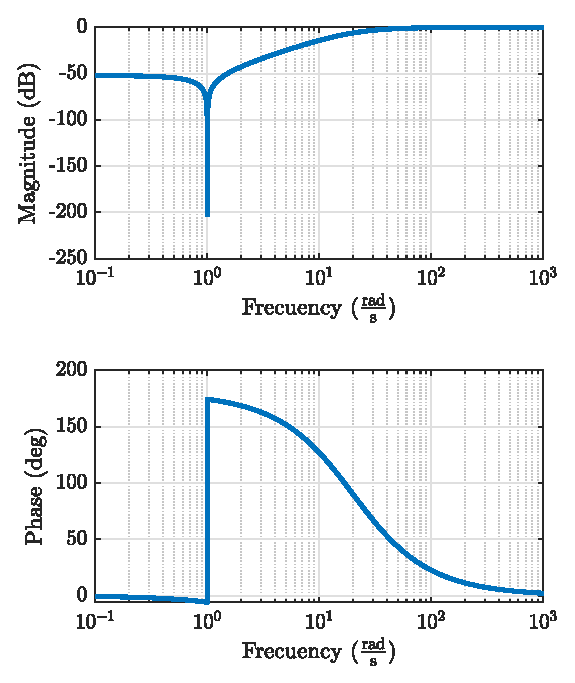
\includegraphics{images/question3/q3_bode_N.eps}
	\caption{Frequency response of Notch filter.}
	\label{fig:notch_filter}
\end{figure}

\newpage
\paragraph{(h)} Figure \ref{fig:q3_CL_N_PD_rlocus} and \ref{fig:q3_CL_N_PD_bode} describe time and frequency response of close-loop system with filter of Notch and proportional-derivative control method. In these figures, time requirements (overshoot $<15\%$ and settling time $<20$ ) and frequency requirements ($PM>50^{\circ}$) are satisfied. After that, proportional-derivative can be computed as $PD = 500 s + 50$. 


\begin{figure}[h!]
	\centering
	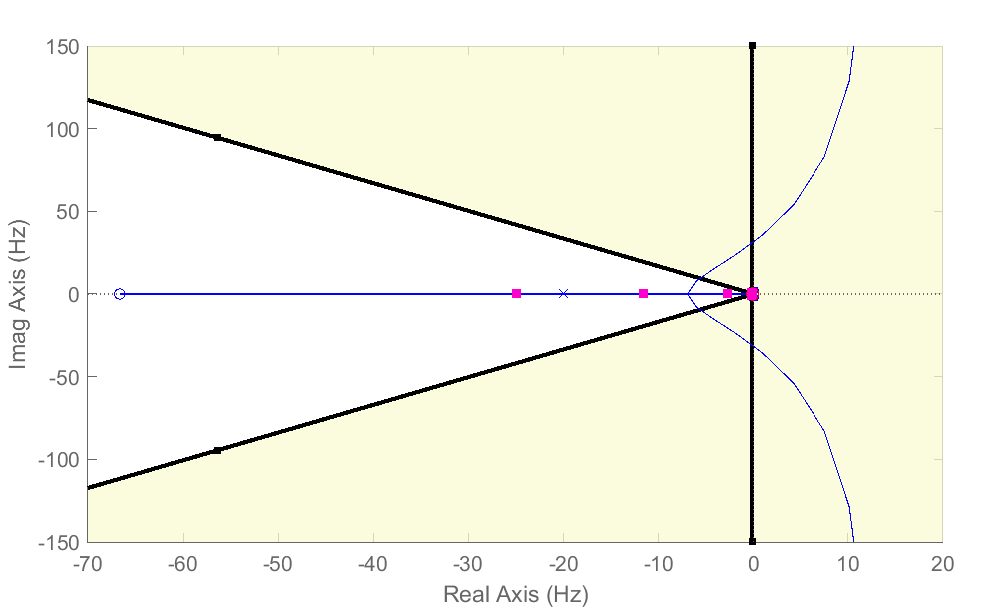
\includegraphics[width=.7\textwidth]{images/question3/sisotool_rlocus.pdf}
	\caption{Close-loop system pole location diagram with filter of Notch and proportional-derivative control method.}
	\label{fig:q3_CL_N_PD_rlocus}
\end{figure}

\begin{figure}[h!]
	\centering
	\subfloat[]{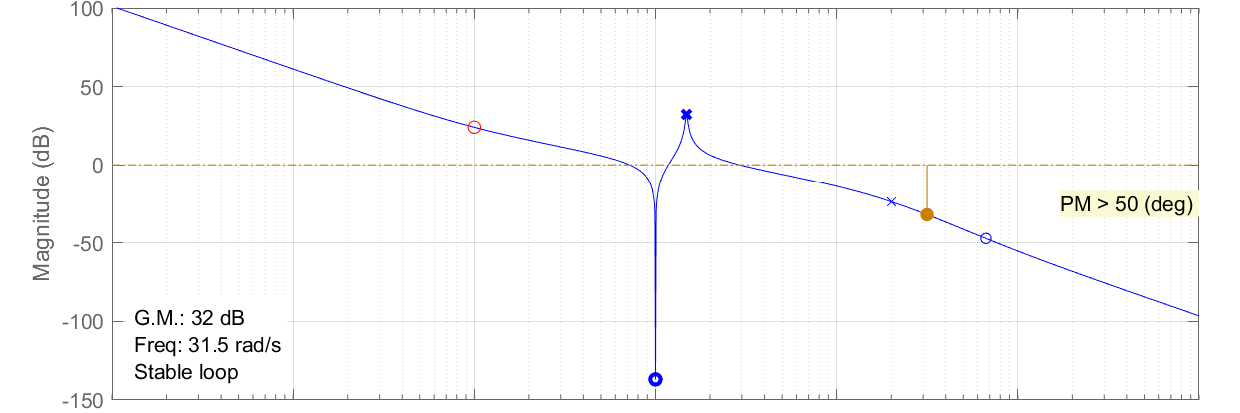
\includegraphics[width=0.85\textwidth]{images/question3/sisotool_bode_1.pdf}}
	\hfill
	\subfloat[]{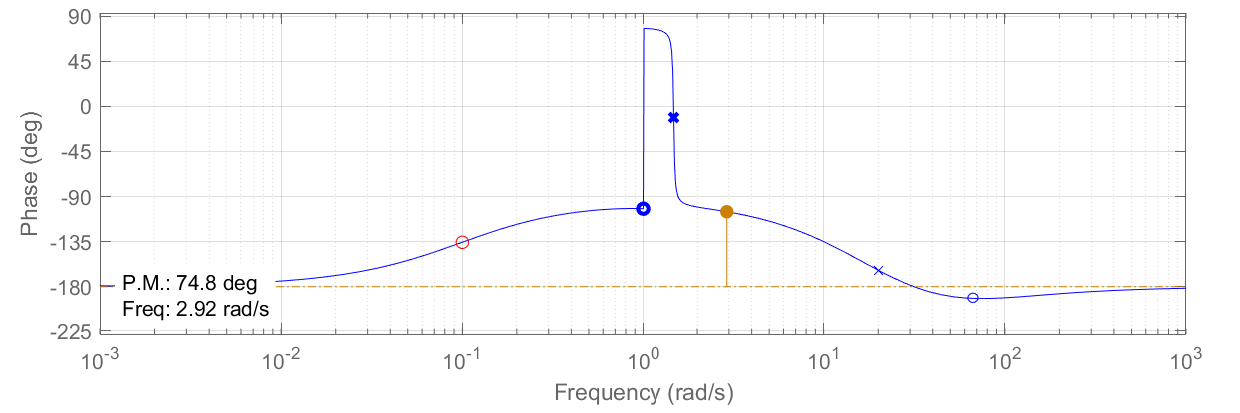
\includegraphics[width=0.85\textwidth]{images/question3/sisotool_bode_2.pdf}}
	\caption{Frequency response of close-loop system with filter of Notch and proportional-derivative control method.}
	\label{fig:q3_CL_N_PD_bode}
\end{figure}

\newpage
\paragraph{(i)} Figure \ref{fig:q3_step_CL_PD_N} describes step response of close-loop system for six different values of stiffness  ($K=10^{-1}[1, 1.4, 1.8, 2.2, 2.6, 3]$ $\mathrm{\frac{N.m}{rad}}$) and damping ($D=10^{-3}[1, 1.8, 2.6, 3.4, 4.2, 5]$ $\mathrm{\frac{N.m.s}{rad}}$).  Hence, system with lower $K$, $D$ (line color blue) have low overshoot and high steady-state error; whereas system with high $K$, $D$ (line color light blue) have high overshoot and low steady-state error.


\begin{figure}[h!]
	\centering
	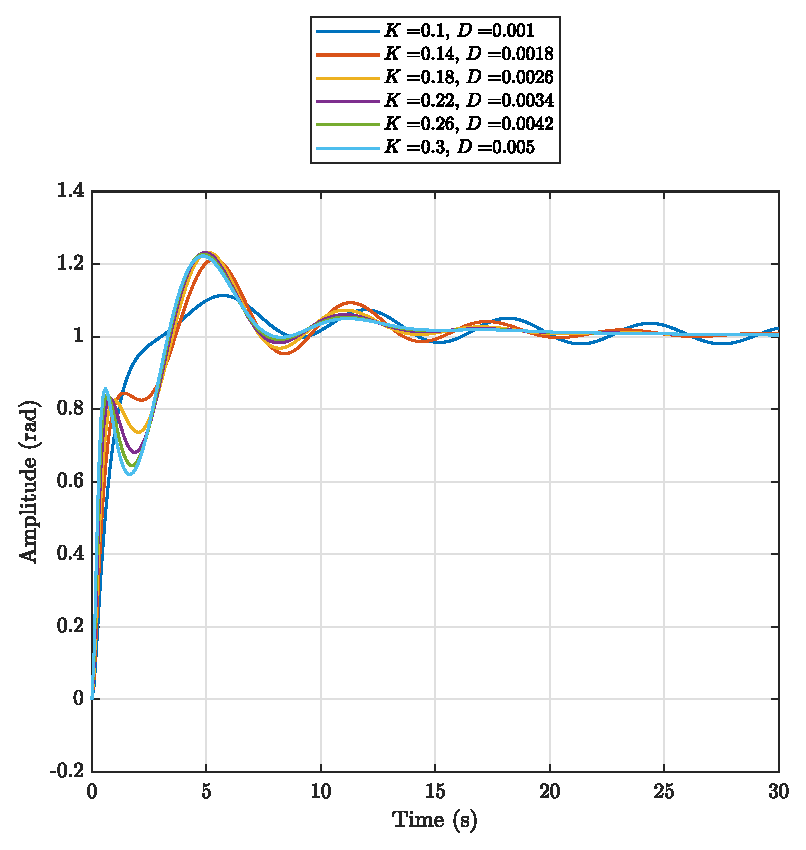
\includegraphics{images/question3/q3_step_CL_PD_N.eps}
	\caption{Step response of close-loop system with filter of Notch and proportional-derivative control method for six different values of stiffness ($K$) and damping ($D$).}
	\label{fig:q3_step_CL_PD_N}
\end{figure}